\newpage
\chapter{Оператори за контрол на изпълнението и потребителски функции}
\label{chapter05}

С процеса на усвояване на софтуерния продукт R всеки потребител установява, че някои команди биват повтаряни многократно. Това навежда на мисълта, че тези команди може да бъдат групирани и съхранени като програмен скрипт (модел на експеримента). Основното предимство на такава организация е възможността един и същи модел да бъде използван са множество експерименти. Второто предимство е, че моделът може да бъде разменян между различни потребители, които работят над същата задача или сходни задачи. Езикът R е в групата на интерпретивните програмни езици, където се намира и програмният език JavaScript. За потребителите познаващи JavaScript, някои конструкции в R биха били изключително познати. 

Скриптовете на R се записват в обикновени текстови файлове с .r разширение, както примерният файл на адрес:

\begin{lstlisting}[caption=Адрес на примерен R скрипт, label=listing0074]
https://raw.githubusercontent.com/TodorBalabanov/Statistical-Data-Processing-with-R/master/code/example0001.r
\end{lstlisting}

Може да се пише с текстов редактор по избор на потребителя, но може да се използва и текстовия редактор към продукта (Фиг. \ref{figure0025}).

\begin{figure}[h!]
  \centering
  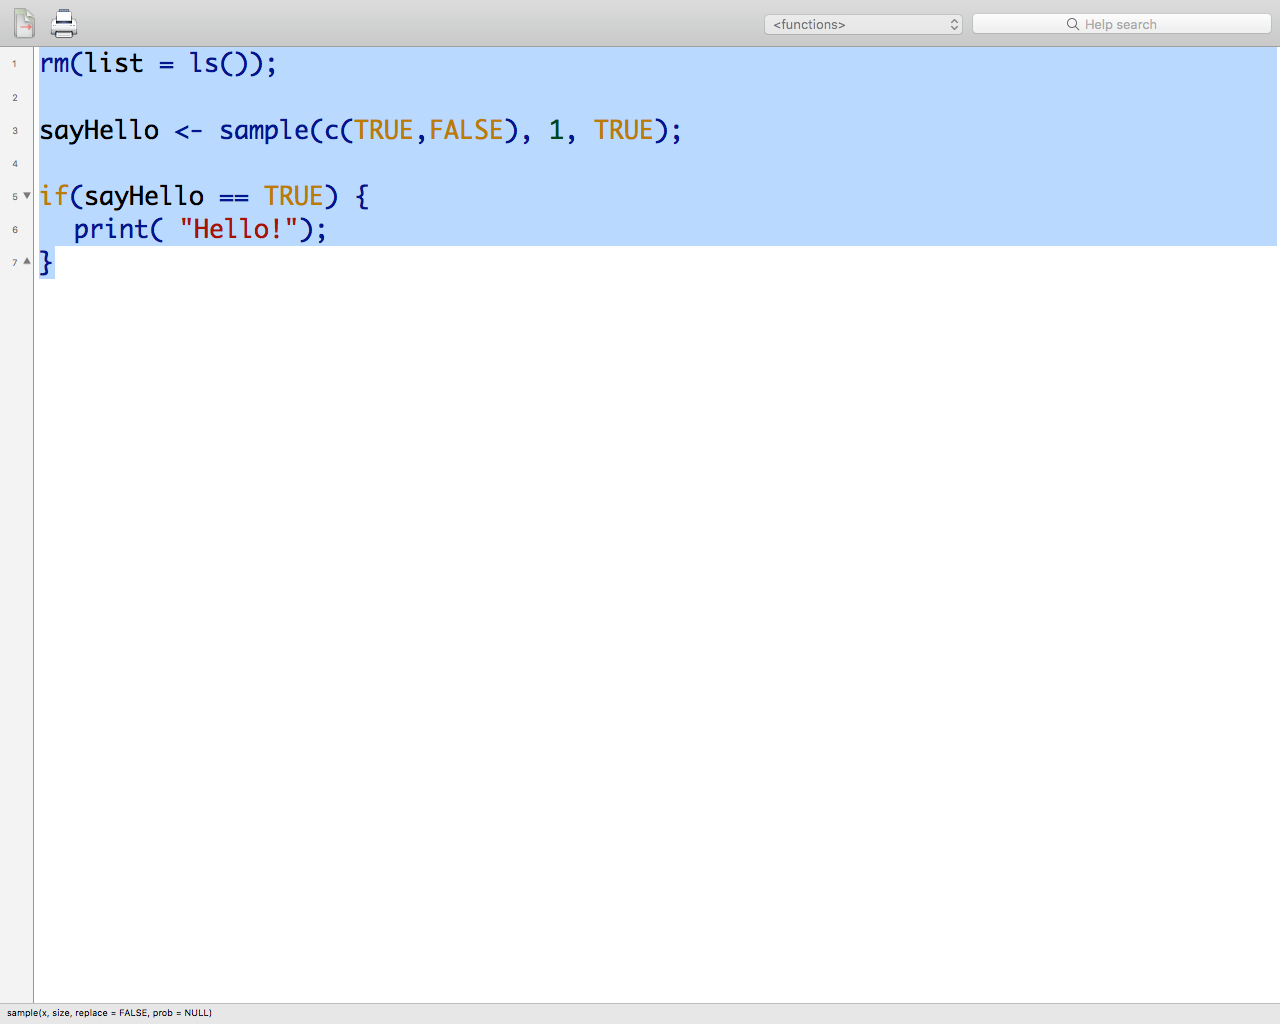
\includegraphics[width=1.0\linewidth]{pic0025}
  \caption{Текстов редактор към продукта R}
\label{figure0025}
\end{figure}
\FloatBarrier

Най-бързият начин за стартиране на скрипта е чрез менюто на вградения текстов редактор Edit->Execute (Фиг. \ref{figure0026}). 

\begin{figure}[h!]
  \centering
  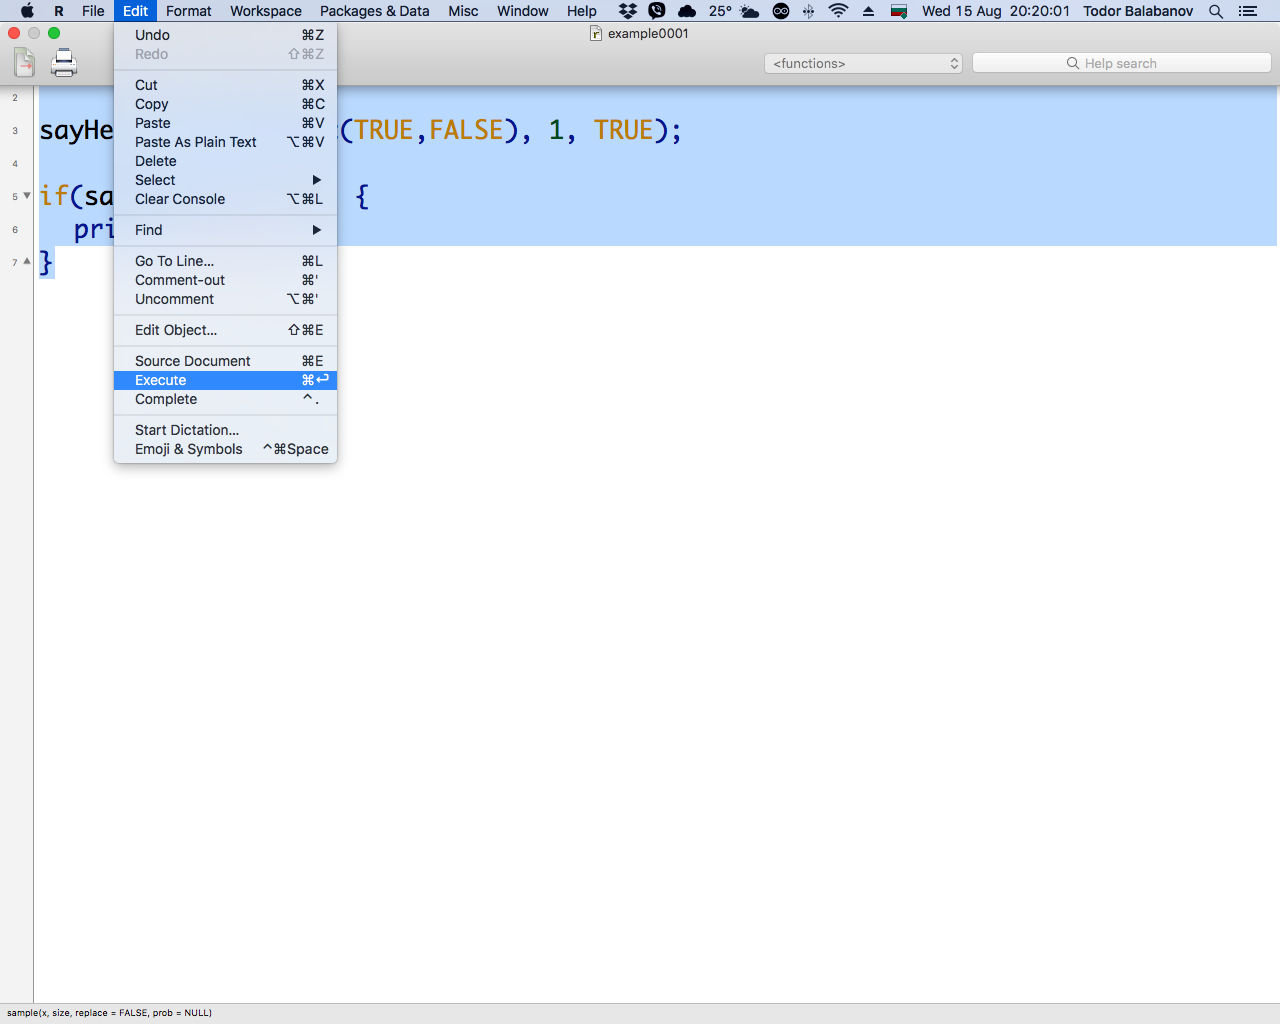
\includegraphics[width=1.0\linewidth]{pic0026}
  \caption{Стартиране на R скрипт}
\label{figure0026}
\end{figure}
\FloatBarrier

Съществено е целият текст на скрипта да бъде маркиран, тъй като командният интерпретатор е оптимизиран в режим за изпълнение на команда по команда. Когато целият скрипт е маркиран се изпълняват, една след друга, всички команди.

\begin{figure}[h!]
  \centering
  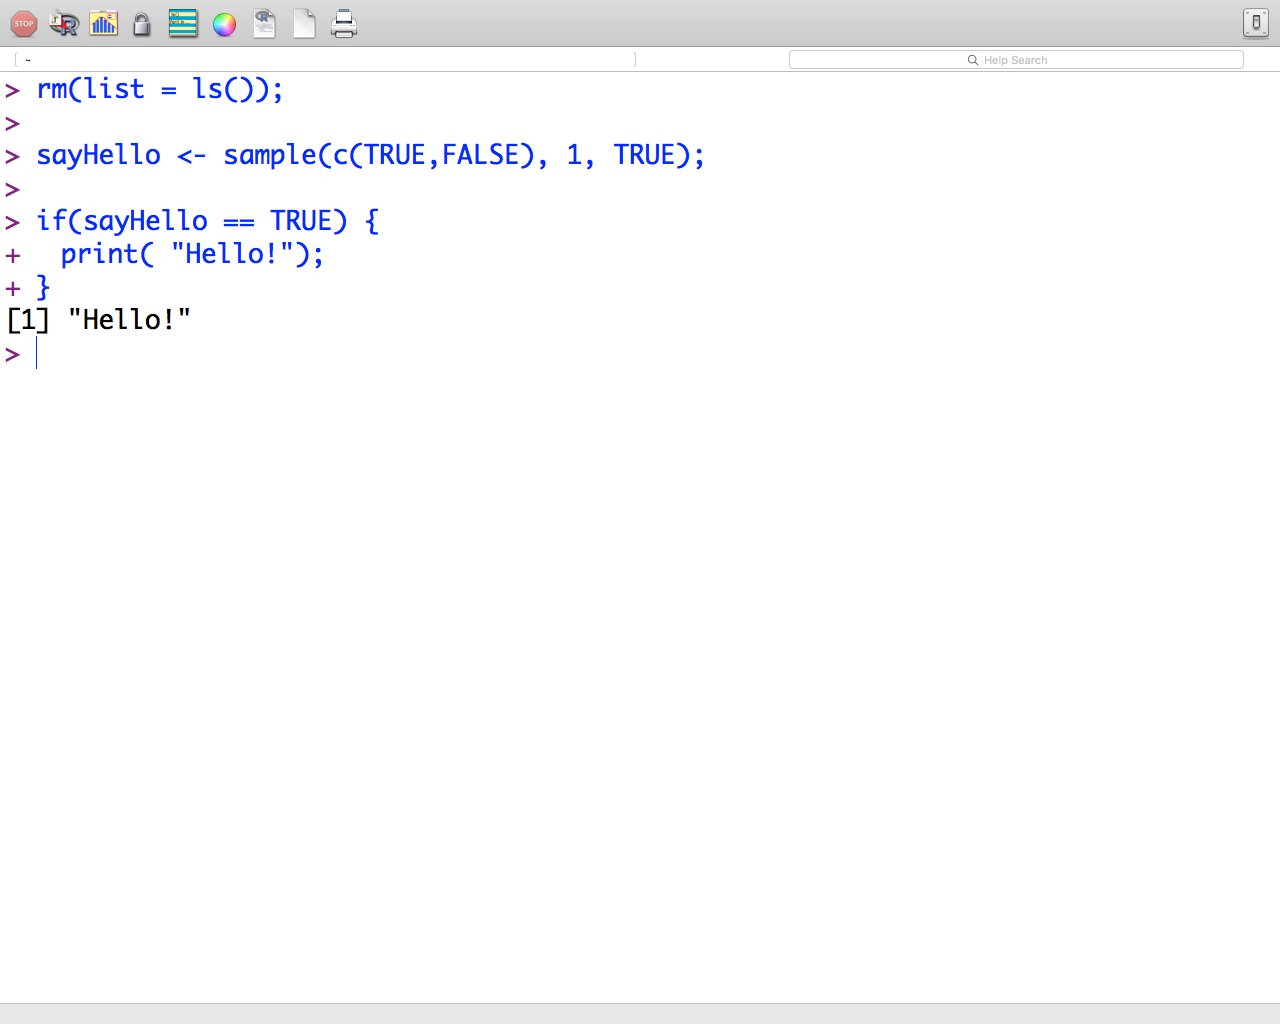
\includegraphics[width=1.0\linewidth]{pic0027}
  \caption{Резултат от изпълнението на R скрипт}
\label{figure0027}
\end{figure}
\FloatBarrier

Резултатът от изпълнението на R скрипта се наблюдава в командния интерпретатор на продукта (Фиг. \ref{figure0027}) и изглежда точно както би трябвало командите да се въведат, на ръка, ако не бяха заредени от скриптов файл.

Програмните скриптове се състоят от последователни инструкции, но с подходящи оператори за преход или повторение изпълнението на командите може да протече в различен от линейния ред. Тази група оператори се нарича оператори за контрол на изпълнението. Общата конструкция на операторите е заглавна част (ключова дума и условие) и тяло. 

\section{Оператори за преход}

Операторите за условен преход променят изпълнението на скрипта в зависимост от логическо или числено условие. От там идва и названието им. В тази група оператори попадат if, else и switch.

\subsection{Оператор за условен преход}

Дори чисто исторически в програмните езици един от първите оператори за преход е оператора за условен преход (if оператор). 

\begin{lstlisting}[caption=Оператор за условен преход if, label=listing0075]
sayHello <- sample(c(TRUE,FALSE), 1, TRUE);

if(sayHello == TRUE) {
	print( "Hello!" );
}

print( "Bye!" );
\end{lstlisting}

Операторът за условен преход използва ключовата дума if (Листинг \ref{listing0075}), а в заглавната му част се записва израз пресмятан до лигическа стойност TRUE или FALSE. Смисълът на оператора if е, че тялото му бива изпълнено единствено ако изчислението на израза в заглавната част доведе до стойност TRUE. Ако изразът в заглавната част бъде изчислено до стойност FALSE, тялото на оператора се пропуска и изпълнението на програмата продължава след него.

В примерът от листинг \ref{listing0075} променливата sayHello получава една случайна логическа стойност (TRUE или FALSE), като двете възможности за равно вероятни. На следващият ред операторът if изписва "Hello!" или го пропуска и изписва "Bye!". Скриптът трябва да се стартира няколко пъти за да се наблюдава ефекта от случайния избор на стойност за променливата sayHello.

\subsection{Алтернатива при условен преход}

\subsection{Каскада от условни преходи}

\subsection{Оператор за многовариантен избор}

